% Options for packages loaded elsewhere
\PassOptionsToPackage{unicode}{hyperref}
\PassOptionsToPackage{hyphens}{url}
\PassOptionsToPackage{dvipsnames,svgnames*,x11names*}{xcolor}
%
\documentclass[
  11pt,
]{article}
\usepackage{lmodern}
\usepackage{setspace}
\usepackage{amsmath}
\usepackage{ifxetex,ifluatex}
\ifnum 0\ifxetex 1\fi\ifluatex 1\fi=0 % if pdftex
  \usepackage[T1]{fontenc}
  \usepackage[utf8]{inputenc}
  \usepackage{textcomp} % provide euro and other symbols
  \usepackage{amssymb}
\else % if luatex or xetex
  \usepackage{unicode-math}
  \defaultfontfeatures{Scale=MatchLowercase}
  \defaultfontfeatures[\rmfamily]{Ligatures=TeX,Scale=1}
\fi
% Use upquote if available, for straight quotes in verbatim environments
\IfFileExists{upquote.sty}{\usepackage{upquote}}{}
\IfFileExists{microtype.sty}{% use microtype if available
  \usepackage[]{microtype}
  \UseMicrotypeSet[protrusion]{basicmath} % disable protrusion for tt fonts
}{}
\makeatletter
\@ifundefined{KOMAClassName}{% if non-KOMA class
  \IfFileExists{parskip.sty}{%
    \usepackage{parskip}
  }{% else
    \setlength{\parindent}{0pt}
    \setlength{\parskip}{6pt plus 2pt minus 1pt}}
}{% if KOMA class
  \KOMAoptions{parskip=half}}
\makeatother
\usepackage{xcolor}
\IfFileExists{xurl.sty}{\usepackage{xurl}}{} % add URL line breaks if available
\IfFileExists{bookmark.sty}{\usepackage{bookmark}}{\usepackage{hyperref}}
\hypersetup{
  pdftitle={Semiparametric estimation for time series: a frequency domain approach based on optimal transportation theory},
  colorlinks=true,
  linkcolor=Maroon,
  filecolor=Maroon,
  citecolor=Blue,
  urlcolor=blue,
  pdfcreator={LaTeX via pandoc}}
\urlstyle{same} % disable monospaced font for URLs
\usepackage[margin=1in]{geometry}
\usepackage{graphicx}
\makeatletter
\def\maxwidth{\ifdim\Gin@nat@width>\linewidth\linewidth\else\Gin@nat@width\fi}
\def\maxheight{\ifdim\Gin@nat@height>\textheight\textheight\else\Gin@nat@height\fi}
\makeatother
% Scale images if necessary, so that they will not overflow the page
% margins by default, and it is still possible to overwrite the defaults
% using explicit options in \includegraphics[width, height, ...]{}
\setkeys{Gin}{width=\maxwidth,height=\maxheight,keepaspectratio}
% Set default figure placement to htbp
\makeatletter
\def\fps@figure{htbp}
\makeatother
\setlength{\emergencystretch}{3em} % prevent overfull lines
\providecommand{\tightlist}{%
  \setlength{\itemsep}{0pt}\setlength{\parskip}{0pt}}
\setcounter{secnumdepth}{5}
\usepackage{caption}
\captionsetup[figure]{font=small}
\ifluatex
  \usepackage{selnolig}  % disable illegal ligatures
\fi
\newlength{\cslhangindent}
\setlength{\cslhangindent}{1.5em}
\newlength{\csllabelwidth}
\setlength{\csllabelwidth}{3em}
\newenvironment{CSLReferences}[2] % #1 hanging-ident, #2 entry spacing
 {% don't indent paragraphs
  \setlength{\parindent}{0pt}
  % turn on hanging indent if param 1 is 1
  \ifodd #1 \everypar{\setlength{\hangindent}{\cslhangindent}}\ignorespaces\fi
  % set entry spacing
  \ifnum #2 > 0
  \setlength{\parskip}{#2\baselineskip}
  \fi
 }%
 {}
\usepackage{calc}
\newcommand{\CSLBlock}[1]{#1\hfill\break}
\newcommand{\CSLLeftMargin}[1]{\parbox[t]{\csllabelwidth}{#1}}
\newcommand{\CSLRightInline}[1]{\parbox[t]{\linewidth - \csllabelwidth}{#1}\break}
\newcommand{\CSLIndent}[1]{\hspace{\cslhangindent}#1}

\title{Semiparametric estimation for time series: a frequency domain
approach based on optimal transportation theory}
\author{Manon Felix\\
Advisor: Prof.~Davide La Vecchia}
\date{May 2021}

\begin{document}
\maketitle
\begin{abstract}
In this master thesis, we develop a novel methodology for estimating
parameters in time series models based on optimal transportation
results. The key idea is to use the Wasserstein distance and Sinkhorn
divergence to derive minimum distance (or divergence) estimators for
short- and long-memory time series models. More precisely, thanks to the
frequency approach, we can compute the distance/divergence between the
empirical distribution of the standardized periodogram ordinates and
their theoretical distribution. To determine the properties of these new
estimators, we perform several Monte-Carlo simulations. Our numerical
results suggest that we have a novel class of root-n consistent minimum
distance estimators. The performance, in terms of Mean Squared-Error, is
similar to the one yielded by the state-of-the-art estimation method
(Whittle's estimator) in the case of short- and long-memory Gaussian
process. Furthermore, when the underlying innovation density of a
long-memory process is skewed, our estimators overperform the Whittle's
estimator.
\end{abstract}

\setstretch{1.5}
\newpage

\tableofcontents

\newpage

\hypertarget{introduction}{%
\section{Introduction}\label{introduction}}

\hypertarget{motivation}{%
\subsection{Motivation}\label{motivation}}

The aim of this master thesis is to combine our knowledge of the optimal
transport theory and the time series analysis in the frequency domain to
develop a novel methodology for estimating the parameters of a process.
We shift away from information divergence-based methods, among which the
standard maximum likelihood estimator approach, and consider instead the
mathematical theory of optimal measure transportation. The optimal
transport theory has been applied in many research areas, especially
machine learning (see e.g.,
\protect\hyperlink{ref-panaretos2019statistical}{Panaretos and Zemel}
(\protect\hyperlink{ref-panaretos2019statistical}{2019})). The
Wasserstein distance has become popular specially for inference in
generative adversarial networks (see e.g.,
\protect\hyperlink{ref-arjovsky2017wasserstein}{Arjovsky, Chintala, and
Bottou} (\protect\hyperlink{ref-arjovsky2017wasserstein}{2017})). To the
best of our knowledge, only a limited number of papers has been
investigating the use of the optimal transport theory in the statistical
analysis of time series analysis (see
\protect\hyperlink{ref-ni2020conditional}{Ni et al.}
(\protect\hyperlink{ref-ni2020conditional}{2020})). Our purpose is to
fill this gap in the literature and study the applicability of the
Wasserstein distance (or, more generally, of some results from optimal
transportation theory) for the statistical analysis of time series, via
frequency domain techniques. The key argument for moving from the time
domain to the frequency domain is that we are dealing with data that are
independent and identically distributed (i.i.d). The assumption of
i.i.d. data facilitates, as it is often the case in statistics, the
estimation of parameters in a model.

We propose a novel class of minimum distance estimator (see
\protect\hyperlink{ref-basu2019statistical}{Basu, Shioya, and Park}
(\protect\hyperlink{ref-basu2019statistical}{2019})) by minimizing the
distance between the theoretical and empirical distribution of the
standardized periodogram ordinates (SPOs). This program is supported by
the fact that the method to replace the maximum likelihood estimator
with minimum Wasserstein distance has already been applied, for instance
in astronomy and climate science (see
\protect\hyperlink{ref-bernton2019parameter}{Bernton et al.}
(\protect\hyperlink{ref-bernton2019parameter}{2019})). Additionally,
consistency properties of estimators based on the Wasserstein distance
has already been studied by
\protect\hyperlink{ref-bassetti2006minimum}{Bassetti, Bodini, and
Regazzini} (\protect\hyperlink{ref-bassetti2006minimum}{2006}) and
\protect\hyperlink{ref-bernton2019parameter}{Bernton et al.}
(\protect\hyperlink{ref-bernton2019parameter}{2019}). In our case, we
study the properties (bias, variance, consistency, etc.) of our new
estimators by means of Monte-Carlo experiments and compare them to the
state-of-the-art estimator, the Whittle's estimator (see
\protect\hyperlink{ref-whittle1953estimation}{Whittle}
(\protect\hyperlink{ref-whittle1953estimation}{1953})). We analyze our
results for several types of distribution (standard, heavy-tailed and
skewed) and focus mainly on large sample sizes to satisfy the i.i.d
conditions. Our results are promising and open the possibility of
further research.

\hypertarget{organization}{%
\subsection{Organization}\label{organization}}

In the first chapter, we review the main concepts of the optimal
transport theory and provide all the distance definitions necessary to
understand the thesis. In the second chapter, we refresh the Whittle's
estimator and all the theoretical results corresponding. Then, we
present the different estimators that we have developed during our
research and compare them to the state-of-art estimator. We end with a
conclusion that contains all the possible research's areas opened up by
this thesis. All the code to reproduce the plots/tables included in this
thesis is available on Github:
\url{https://github.com/ManonFelix/Semidiscrete_estimation_ts}.

\hypertarget{measure-transportation}{%
\section{Measure transportation}\label{measure-transportation}}

This chapter aims to explain the main principles behind the theory of
optimal transport. The original formulation of the optimal transport
problem was given by \protect\hyperlink{ref-monge1781memoire}{Monge}
(\protect\hyperlink{ref-monge1781memoire}{1781}). He proposed a way to
calculate the most effective strategy for moving a large amount of sand
from one place to another with the least amount of effort required. In
mathematical terms, given a source measure \(\mu\), target measure
\(\nu\) supported on sets \(X\) and \(Y\) respectively and a
transportation cost function \(c(x,y)\) the goal is to find a transport
map \(T:X \rightarrow Y\) such as

\[\min _{\nu=T_{\#} \mu} \int_{X} c(x, T(x)) \mathrm{d} \nu(x)\]

where the constraint
\(\mu(T^{-1}(A) = \nu(A) \implies \nu=T_{\#} \mu \ , \forall A\) ensures
that all the mass from \(\mu\) is transported to \(\nu\) by the map
\(T\). The notation \(\nu=T_{\#} \mu\) means that the map \(T\) pushes
forward \(\mu\) to a new measure \(\nu\) and therefore \(T_{\#}\) is
called the pushforward operator. A generalization of this problem was
proposed by
\protect\hyperlink{ref-kantorovich1942translocation}{Kantorovich}
(\protect\hyperlink{ref-kantorovich1942translocation}{1942}). In his
reformulation, he seeks for a transport plan and allows mass splitting.
We therefore compute how much mass gets moved from \(x\) to \(y\) and
store the results in a measure
\(\pi \in \mathcal{P}\left(\mathbb{R}^{d}, \mathbb{R}^{d}\right)\) which
satisfies for all \(A, B \in \mathcal{B}\left(\mathbb{R}^{d}\right)\):
\(\pi\left(A \times \mathbb{R}^{d}\right)=\mu(A), \ \pi\left(\mathbb{R}^{d} \times B\right)=\nu(B).\)
We denote by \(\Pi(\mu, \nu)\) the set of transport plans between
\(\mu\) and \(\nu\) (i.e.~couplings). Then, the Kantorwich or
p-Wasserstein distance is defined as

\begin{equation}
W_{p}(\mu, \nu)=\left(\min _{\pi \in \Pi(\mu, \nu)} \int_{\mathbb{R}^{d} \times \mathbb{R}^{d}}|x-y|^{p} d \pi(x, y)\right)^{\frac{1}{p}}.
\end{equation}

The case of one dimensional probability densities, say \(f_S(x)\) and
\(f_T(y)\) with cumulative distribution functions \(F_S(x)\) and
\(F_T(x)\), is specifically interesting as the Wasserstein distance
(a.k.a the Earth Mover's Distance (EMD)) has a closed-form solution

\begin{equation}
\mathcal{W}_{1}(\mu, \nu)=\int_{\mathbb{R}}\left|F_{\mu}(t)-F_{\nu}(t)\right| d t
\label{eq:wass_1}
\end{equation}

The possibility of using this closed formed solution to conduct
inference on time series motivated the thesis.

Solving the Eq. \ref{eq:wass_1} can be computationally expensive. To
prevent this inconvenient problem,
\protect\hyperlink{ref-cuturi2013sinkhorn}{Cuturi}
(\protect\hyperlink{ref-cuturi2013sinkhorn}{2013}) introduced a modified
version of the Wasserstein distance:

\begin{equation}
W_{\lambda}(\mu, \nu) =\int_{x, y} C(x, y) \mathrm{d} \pi(x, y)+ \varepsilon \int \log \left(\frac{\pi(x, y)}{\mathrm{d} \mu(x) \mathrm{d} \nu(y)}\right) \mathrm{d} \pi(x, y). 
\label{eq:sink}
\end{equation}

Minimizing Eq. \ref{eq:sink} leads to the so called Sinkhorn divergence.
This divergence is obtained adding to the original optimal
transportation problem an entropic regularization term (right part).
When \(\lambda\) is small, the Sinkhorn divergence approximates the
Wasserstein distance. In contrast to the Wasserstein distance, the
regularized Sinkhorn divergence is differentiable and smooth.

In this thesis, we use all the concepts presented in this section in
order to establish new minimum distance estimators in time series
analysis.

\hypertarget{inference-in-the-frequency-domain}{%
\section{Inference in the frequency
domain}\label{inference-in-the-frequency-domain}}

Before introducing our estimators, let us first provide an overview of
the theory that is commonly applied to conduct inference in the
frequency domain.

Consider a stationary process \(\{Y_t\}\) of \(n\) observations
\(y_{1:n} = y_1, … ,y_n\). During our research project, we study linear
stochastic process \(\{Y_t\}\) satisfying

\[
\phi(L)(1-L)^{d} Y_{t}=\varphi(L) \epsilon_{t}
\]

where \(LX_t = X_{t-1}\) (back shift operator). \(\phi(z)\) and
\(\varphi(z)\) are the auto-regressive and moving average polynomial of
order \(p\) and \(q\) respectively. The time series \(\{Y_t\}\) may or
may not have long memory depending on the value of \(d\). When
\(0 < d < 0.5\) the process is called a long-memory process and are
extensively applied in finance (see e.g
\protect\hyperlink{ref-tsay2005analysis}{Tsay}
(\protect\hyperlink{ref-tsay2005analysis}{2005})) . In the literature,
we often rewrite \(d\) as \(H = d - 0.5\). In our research, we do not
assume any distribution for the innovation term \(\epsilon_t\). We
present our results for the case when
\(\epsilon_t \sim N(0,\sigma^2_\epsilon =1)\) but also underlying
innovation densities with fatter tails (like e.g.~Skew t (see
\protect\hyperlink{ref-azzalini2003distributions}{Azzalini and
Capitanio} (\protect\hyperlink{ref-azzalini2003distributions}{2003}))
and Student t).

To conduct inference on the model parameters
\(\theta=\left(\sigma_{\epsilon}^{2}, d, \phi_{1}, \ldots, \phi_{p}, \varphi_{1}, \ldots, \varphi_{q}\right)\)
of long-memory processes, we could assume that \(\epsilon_t\) is
normally distributed. Thanks to this assumption, we can write the
likelihood of the process and optimize it to find \(\hat \theta\).
Nevertheless, this approach is extremely time-consuming and can even be
unfeasible due to the strong dependence and long-memory properties of
the process. Instead, we can approach the problem in the frequency
domain and work on Fourier frequencies rather than time data. The
frequency domain approach represents a time series into combination of
sinusoids.

The main tool utilized in the frequency domain is the spectral density.
The spectral density \(f(\lambda_j, \theta)\) of \(Y_t\)

\[
f(\lambda_j, \theta)=\left|1-e^{i \lambda}\right|^{-2 d}\frac{\sigma_{\epsilon}^{2}}{2 \pi} \frac{|\varphi(\exp \{-i \omega\})|^{2}}{|\phi(\exp \{-i \omega\})|^{2}}
\] where \(\varphi(x)=1-\sum_{k=1}^{p} \varphi_{k} x^{k}\) and
\(\phi(x)=1+\sum_{k=1}^{q} \phi_{k} x^{k}\). \(\lambda_j\) are the
fundamental Fourier frequencies where
\(\lambda_j=2 \pi(j / n), j \in \mathcal{J}=\{1,2, \ldots,[(n-1) / 2]\}\).
The spectrum of a time series can be estimated by the method of moment.
Its sample analogue is called the periodogram
\(I\left(\lambda_{j}\right)=\frac{1}{2 \pi n}\left|\sum_{t=1}^{n}\left(Y_{t}-\bar{Y}_{n}\right) e^{i t \lambda_{j}}\right|^{2}\).
The periodogram is asymptotically unbiased. Nevertheless, it is an
inconsistent estimator. An important and key result showed by
\protect\hyperlink{ref-priestley1981spectral}{Priestley}
(\protect\hyperlink{ref-priestley1981spectral}{1981}) and
\protect\hyperlink{ref-brillinger2001time}{Brillinger}
(\protect\hyperlink{ref-brillinger2001time}{2001}) is that the
periodogram ordinates are asymptotically independent and exponentially
distributed with rate equal to the spectral density. In other words, the
standardized periodogram ordinates are asymptotically independent and
have an exponential distribution with rate one. Therefore, in 1953,
\protect\hyperlink{ref-whittle1953estimation}{Whittle}
(\protect\hyperlink{ref-whittle1953estimation}{1953}) had the idea to
minimize the Whittle approximated likelihood:

\begin{equation}
L_{W}(\theta)=\frac{1}{2 \pi}\left[\int_{-\pi}^{\pi} \ln f(\lambda, \theta) d \lambda+\int_{-\pi}^{\pi} \frac{I(\lambda)}{f(\lambda, \theta)} d \lambda\right]
\label{eq:Whittle}
\end{equation}

which is derived from the fact that the SPOs are asymptotically
identically distributed according to an exponential distribution. Eq.
\ref{eq:Whittle} can be rewritten by separating the variance component
from the rest of the parameters vector as

\begin{equation}
L_{W}\left(\theta^{*}\right)=\sum_{j \in \mathcal{J}} \frac{I\left(\lambda_{j: n}\right)}{f\left(\lambda_{j: n}, \theta^{*}\right)}
\end{equation}

where
\(f\left(\lambda_{j: n}, \theta^{*}\right)=2 \pi \sigma_{\epsilon}^{2} f\left(\lambda_{j: n}, \theta^{*}\right)\)
and
\(\theta^{*}=(1, \eta = \left(d, \phi_{1}, \ldots, \phi_{p}, \varphi_{1}, \ldots, \varphi_{q}\right))\).

Finally, \protect\hyperlink{ref-beran1994statistics}{Beran}
(\protect\hyperlink{ref-beran1994statistics}{1994}) suggests the
following minimization problem. Firstly, minimize
\(\arg \min _{\eta} L_{W}\left(\theta^{*}\right)=\arg \min _{\eta} L_{W}(\eta)\)
which yields to \(\hat{\eta}\). Secondly, set
\(\hat{\sigma}_{\epsilon}^{2}=2 \pi L_{W}(\hat{\eta}).\) The author
demonstrates the consistency of the parameter \(\hat \theta^*\).
Additionally, the parameter is \(\sqrt{n}\)-consistent and converges to
a normal distribution. In the case of underlying Gaussian innovation
terms, \(\hat \theta\) achieves the Cramer-Rao lower bound.

The Whittle's estimator can also be applied for ARIMA(\(p,q\)) process
and remains \(\sqrt{n}\)-consistent and normally distributed. We
therefore use this parameter as our reference to compare our results as
it is still the state-of-the-art methodology.

\hypertarget{methodology}{%
\section{Methodology}\label{methodology}}

\hypertarget{problem-settings}{%
\subsection{Problem settings}\label{problem-settings}}

Our goal is to find the parameter \(\eta = \theta^*\) of a time series
model in the parameter space \(\theta^* \in \mathcal{H}\) with dimension
\(\mathcal{H} \subset \mathbb{R}\) that minimizes the distance between
the empirical and theoretical cumulative distributions of the SPOs. We
denote the distance or divergence used by \(\mathcal{D}\) and write our
minimum distance estimator such as

\[\hat{\theta^*}=\underset{\theta^* \in \mathcal{H}}{\operatorname{argmin}} \ \mathcal{D}\left({\mu}, \nu\right) .\]
where \(\mu\) is the theoretical exponential distribution and \(\nu\) is
the empirical distribution of the SPOs. In our study, several estimators
are proposed and therefore \(\mathcal{D}\) is redefined for each
optimization problem. For instance, when \(\mathcal{D}\) is the
Wasserstein distance, we denote the corresponding minimum Wasserstein
estimator (MWE) as \(\hat \theta^*_{MWE}\). During our research, we
always assumed the variance of the innovation term \(\sigma^2_\epsilon\)
to be known and equal to one. Hence, our parameter vector to be
estimated is
\(\theta^* = (d, \phi_{1}, \ldots, \phi_{p}, \varphi_{1}, \ldots, \varphi_{q})\).
In addition to that, we focus first on processes with underlying
Gaussian distribution and then extend to other distributions whith
fatter tails.

\newpage

\hypertarget{estimation-methods}{%
\subsection{Estimation methods}\label{estimation-methods}}

\hypertarget{minimum-wasserstein-estimator}{%
\subsubsection{Minimum Wasserstein
Estimator}\label{minimum-wasserstein-estimator}}

Recap that the Wasserstein distance when \(p = 1\) is given by:

\begin{equation}
\mathcal{W}_{1}(\mu, \nu)=\int_{\mathbb{R}}\left|F_{\mu}(t)-F_{\nu}(t)\right| d t.
\end{equation}

\(F_\nu\) being the empirical cumulative distribution of the SPOs, we
estimate it by
\(\hat F_\nu(x) = \frac{1}{m} \sum_{j=1}^{m} \mathbf{1}_{X_{j} \leq x}\)
where \(x_j\) are the SPOs of a time series process asymptotically
exponentially distributed. To compute \(F_\mu\), as it is common in
machine learning literature about generative models, we initially
thought to generate exponential random variables and stack then in a
vector. In mathematical terms, for a sample size \(n\), we generate a
vector of length \((n-1)/2 = m\) containing random variables following
an exponential distribution with rate one. Since \(p = 1\), the
Wasserstein distance can be approximated by

\begin{equation}
\mathcal{D}(\mu, \nu) = \frac{1}{m} \sum_{j = 1}^{m} |x_j - z_j| 
\label{eq:wass_1_app}
\end{equation}

where \(x_j\) are the SPOs of a time series process asymptotically
exponentially distributed and \(z_j\) are the observations generated
according to \(Z \sim Exp(1)\). Minimizing Eq. \ref{eq:wass_1_app} leads
to the minimum Wasserstein estimator noted
\(\hat \theta^*_{MWE} = argmin \  \mathcal{D}(\mu, \nu)\).

Figure \ref{fig:wasserstein_farima} displays the Wasserstein loss
function of two FARIMA(\(0,d,0\)) processes. The top plot shows a smooth
and concave loss function with a global minimum that is the same value
as the Whittle's estimator's. On the other hand, the lower shows a
wiggly function around the true value of the parameter. Thus, if one
uses the Wasserstein loss to estimate a parameter, these two phenomena
arise: we end up with either a smooth function containing a global
minimum or a function that fluctuates and has several local minima.
Through this thesis, we present several estimators that aim to provide
more reliable loss functions.

Our first finding is that the computed distance might vary widely around
the true parameter value and its value depends heavily on the sample
\(z_1, ..., z_m\) simulated from an Exp(1). As a consequence, the
estimated model parameter(s) \(\hat \theta_{MWE}\) showed a strong
dependence on the random exponential variables generated. In Figure
\ref{fig:wasserstein_z} we continue with the process used to plot the
second line on Figure \ref{fig:wasserstein_farima} and simply change the
seed with which the vector \(Z_j\) is generated. We remark that we are
now dealing with a loss function that is smooth and has a global minimum
that is precisely the true value of the parameter \(\theta = H = 0.8\).
Concretely, by modifying the vector \(Z_j\), we can obtain a more
appropriate loss function. However, by definition a random vector cannot
be controlled.

\hfill\break

\begin{center}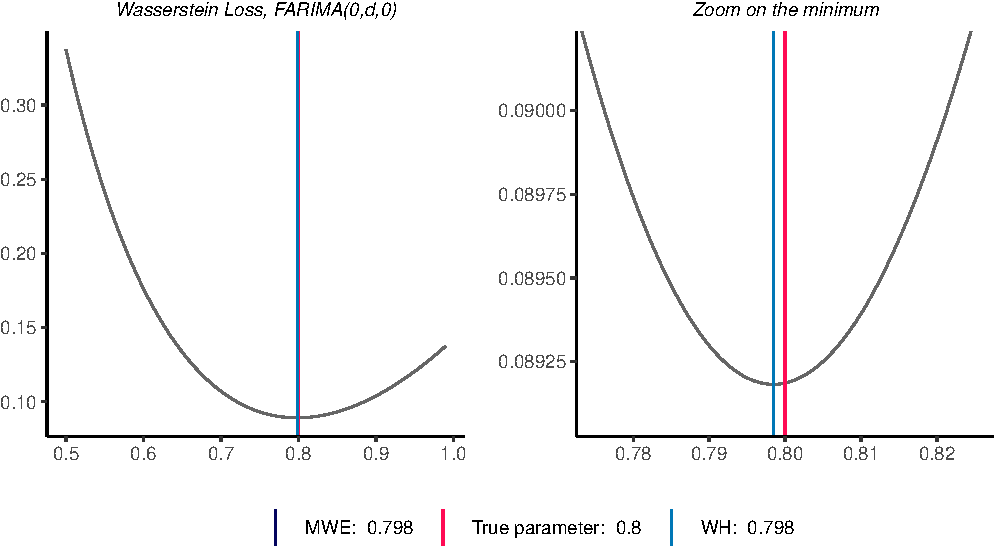
\includegraphics[width=0.6\linewidth]{Master_thesis_V1_files/figure-latex/unnamed-chunk-2-1} \end{center}

\begin{figure}[h]

{\centering 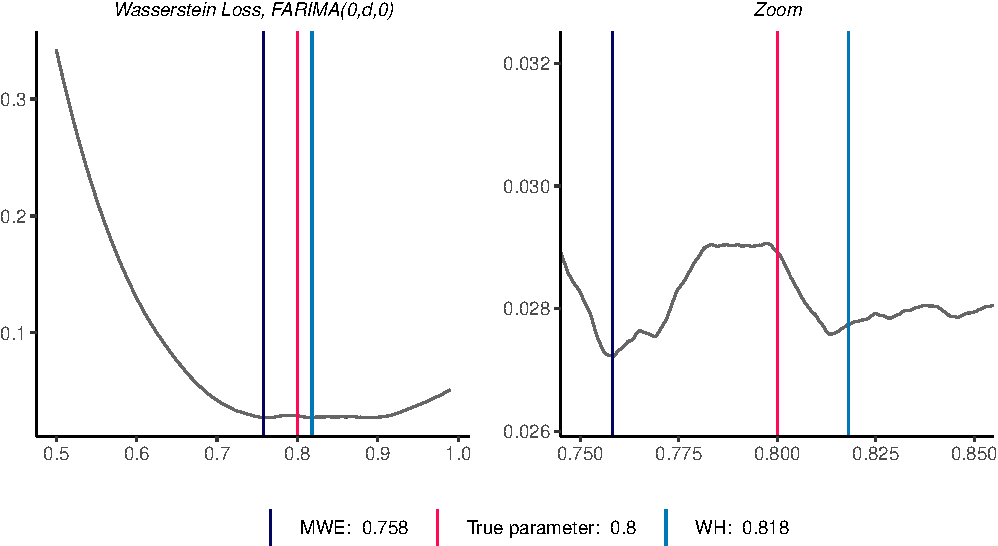
\includegraphics[width=0.6\linewidth]{Master_thesis_V1_files/figure-latex/wasserstein_farima-1} 

}

\caption{Wasserstein loss functions of two FARIMA(0,d,0) processes where H = 0.8 (d = 1.2). The sample size is 3001. The left column display the entire loss functions for all possible parameter values that a long-memory process can take (0.51 < H < 0.99). The right column is a zoom on the functions.}\label{fig:wasserstein_farima}
\end{figure}

\begin{figure}[h]

{\centering 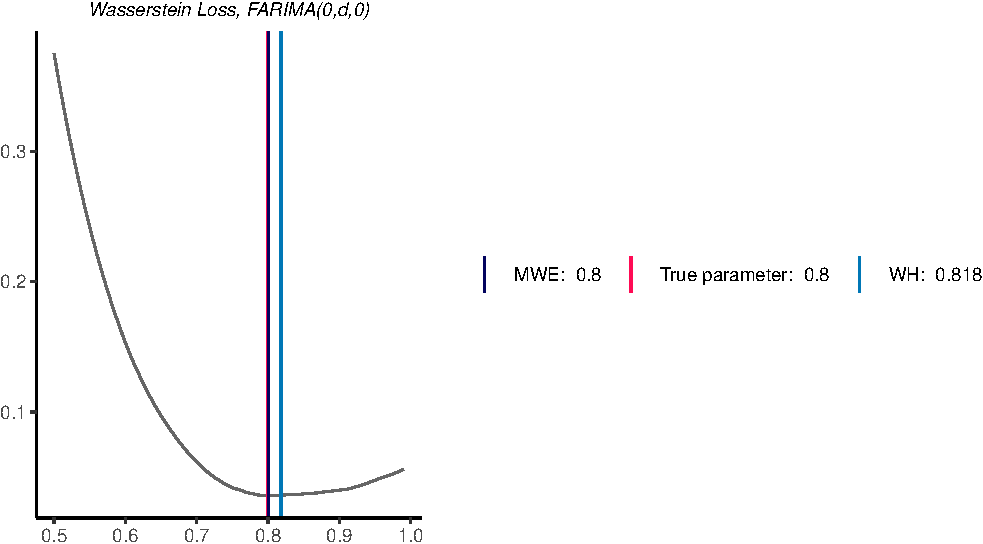
\includegraphics[width=0.55\linewidth]{Master_thesis_V1_files/figure-latex/wasserstein_z-1} 

}

\caption{Wasserstein loss function of the FARIMA(0,d,0) process (bottom one) of Figure 1 computed with another random vector.}\label{fig:wasserstein_z}
\end{figure}

In order to get a better overview of the behavior of the MWE when the
vector \(Z_j\) changes, we compute \(k = 200\) times
\(\hat \theta^*_{MWE}\) for a given process. Then, we plot them for
different sample sizes in Figure \ref{fig:MWE_n}. We can observe that,
for a small sample size, the estimated parameter depends heavily on the
random vector \(Z_j\). Nevertheless, the mean remains relatively close
to the true value. As the sample size increases, the mean of the minimum
Wasserstein estimators \(\hat \theta^*_{MMWE}\) concentrates around the
true parameter value.

\begin{figure}[h]

{\centering 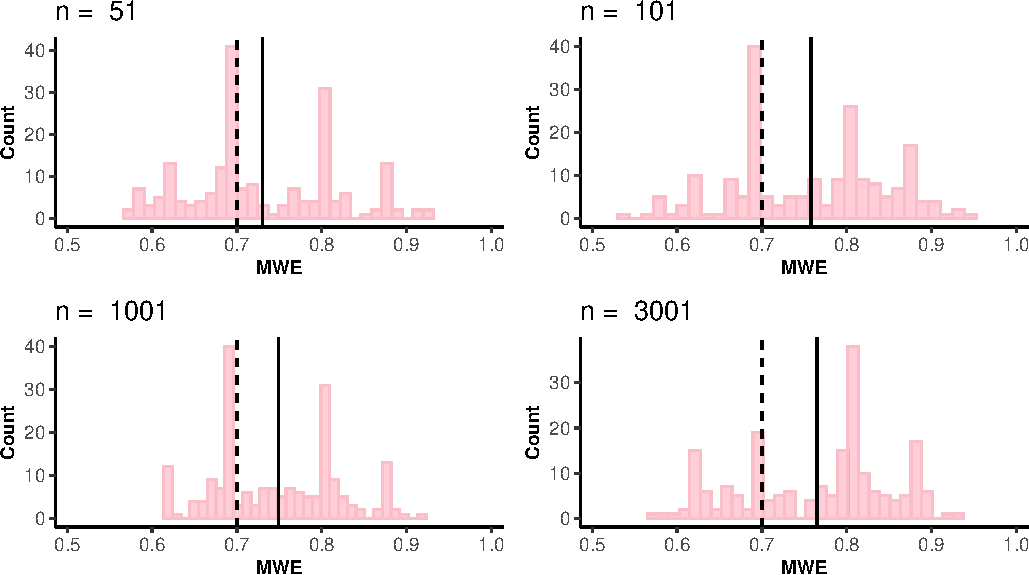
\includegraphics[width=0.7\linewidth]{Master_thesis_V1_files/figure-latex/MWE_n-1} 

}

\caption{Four different FARIMA(0,d,0) processes for different sample sizes (n = 51, 101, 1001 and 3001). For the same process, we simulate 200 vectors following an exponential distribution and then compute the MWE. The figure represents the four histograms of the MWE. The dashed line is the true parameter H = 0.7 value and the full line is the mean of the MWE.}\label{fig:MWE_n}
\end{figure}

To cope with this problem of dependence between the random vector
\(Z_j\) and the parameter estimate, we are going to explore two options.

\hypertarget{mean-of-minimum-wasserstein-estimators}{%
\subsubsection{Mean of Minimum Wasserstein
Estimators}\label{mean-of-minimum-wasserstein-estimators}}

Option A: for the simulated times series, we generate several
exponential random variables and stack them in vectors. Then, we
estimate the model parameter for each of the simulated vector and report
the mean of the estimated parameter. For illustration, based on the same
process than in Figure \ref{fig:MWE_n} with \(n = 3001\), we generate
\(k = 10, 20 , 50, 100 , 200, 500, 1000\) random vectors, estimate the
\(k\) parameters and then report the mean. Thus, the mean becomes our
estimator and we note it \(\hat \theta^*_{MMWE}\). The results are
listed in Table \ref{tab:MWE_k}. As \(k\) increases, the average becomes
progressively closer to the true parameter.

\begin{table}[h]
\centering
\begin{tabular}{|c|c|c|c|c|c|c|c|c|}
\hline
k &  1 & 10   & 20    & 50    & 100   & 200   & 500   & 1000 \\
\hline
MWE & 0.807 & 0.73 & 0.727 & 0.726 & 0.721 & 0.719 & 0.714 & 0.714 \\
\hline
\end{tabular}
\caption{Mean of the minimum Wasserstein estimators for a FARIMA($0,d,0$) of size $n = 3001$ by varying the value of $k$, i.e. the number of exponential random vectors generated. The true value is 0.7.}
\label{tab:MWE_k}
\end{table}

\hypertarget{minimum-semidiscrete-wasserstein-estimator}{%
\subsubsection{Minimum Semidiscrete Wasserstein
Estimator}\label{minimum-semidiscrete-wasserstein-estimator}}

Option B: instead of using the empirical cumulative distribution
function (c.d.f) of exponential random variables generated from a
computer, we plan to use the c.d.f of exponential variables with rate
one for the SPOs, namely \(F(x)=1-e^{-x}\). Therefore, the Wasserstein
distance becomes:

\begin{equation}
\int_\mathcal{X}\left|\hat F(x)- (1 - e^{-x})\right| \mathrm{d} x 
\end{equation}

where \(\hat F(x) = \frac{1}{m} \sum_{j=1}^{m} 1_{X_{j} \leq x}\) and
\(x_j\) are the SPOs of a process. To compute this distance, we replace
\(\hat F_\mu(z) = \frac{1}{m}\sum_{j=1}^{m} \mathbf{1}_{Z_{j} \leq z}\)
by \(F_\mu = 1 - e^{-x}\). We use a trapezoidal integration to
approximate the integral. Thanks to this second option, there is no
longer randomness in our process estimation.

Still, another problem persists. The Wasserstein loss, even for large
sample size, is often not well-shaped (i.e smooth and concave): it may
contain several local minima (see e.g.~Figure
\ref{fig:wasserstein_farima}). This concern leads to biased estimates
with large variance. It should also be noted that the loss shape
degenerates even more when n decreases (see Figure
\ref{fig:small_sample}). So far, we are not able to explain why there is
such diversity in the shape of the loss functions.

\begin{center}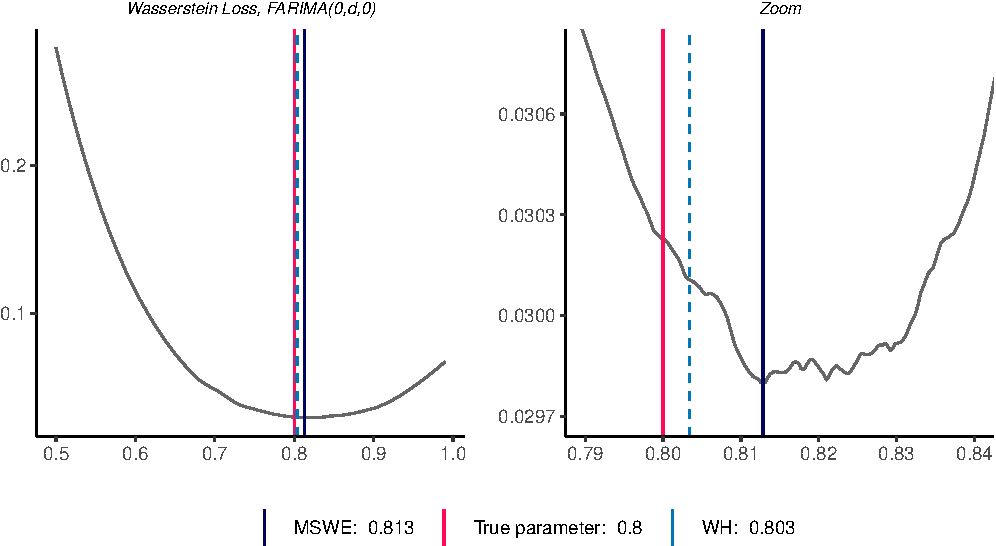
\includegraphics[width=0.6\linewidth]{Master_thesis_V1_files/figure-latex/unnamed-chunk-3-1} \end{center}

\begin{figure}

{\centering 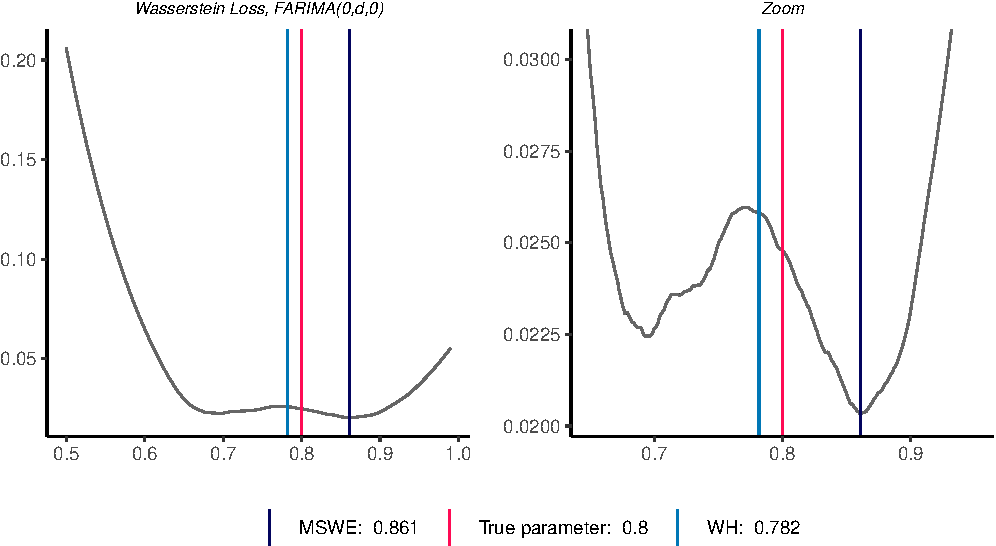
\includegraphics[width=0.6\linewidth]{Master_thesis_V1_files/figure-latex/semi_wass-1} 

}

\caption{Semidiscrete Wasserstein loss functions for two FARIMA(0,d,0) processes. The sample size is 3001 and the true parameter value is 0.8.}\label{fig:semi_wass}
\end{figure}

\begin{figure}

{\centering 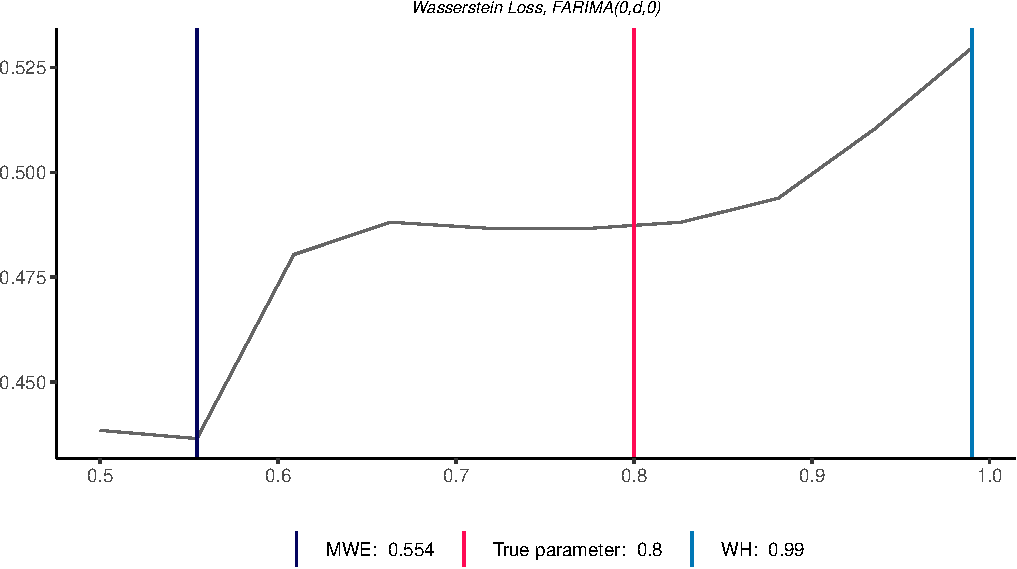
\includegraphics[width=0.6\linewidth]{Master_thesis_V1_files/figure-latex/small_sample-1} 

}

\caption{Wasserstein loss function for a small sample size (n = 21) FARIMA(0,d,0) process.}\label{fig:small_sample}
\end{figure}

\hypertarget{minimum-weighted-wasserstein-estimator}{%
\subsubsection{Minimum Weighted Wasserstein
Estimator}\label{minimum-weighted-wasserstein-estimator}}

After searching a way to fix this problem, we found that by putting some
weights in the loss function defined by the Wasserstein distance, we
obtain a much more regular optimization problem. Therefore, we seek the
parameter that minimizes

\begin{equation}
\mathcal{W}_{1}(\mu, \nu)=\int_{\mathbb{R}}\left|F_{\mu}(t)-F_{\nu}(t)\right| d t
\end{equation}

where the empirical cumulative distribution of the SPOs is
\(\hat F_\nu(x)=\sum_{i=1}^{m} w_{j} 1\left\{X_{i} \leq x\right\}\) and
the weights \(w_j\) are

\begin{equation}
w_j = \frac{\frac{I(\lambda_j)}{f(\lambda_j; \theta)}}{\sum^m_{j = 1}\frac{I(\lambda_j)}{f(\lambda_j; \theta)}}
\label{eq:weights}
\end{equation}

The employment conditions of R packages to calculate the distances used
in this thesis required that the weights sum to \(1\) and that are
comprised between \(0\) and \(1\). Therefore, our first intuition is to
use the weights proposed in Eq. \ref{eq:weights}.

Figure \ref{fig:weighted_wasserstein} shows the same process and vector
\(Z_j\) as Figure \ref{fig:wasserstein_farima} and the same vector
\(Z_j\) but applies the weights to calculate our weighted Wasserstein
distance. We can observe that the weighted Wasserstein loss function is
immediately smoother and contains a minimum which is even closer to the
true parameter than the Whittle's estimator.

\begin{figure}

{\centering 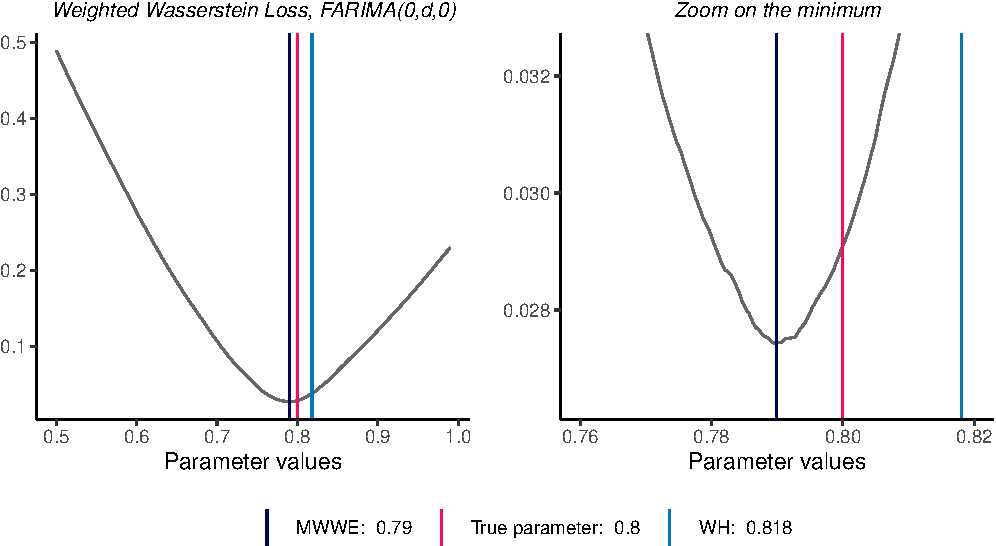
\includegraphics[width=0.75\linewidth]{Master_thesis_V1_files/figure-latex/weighted_wasserstein-1} 

}

\caption{Weighted Wasserstein loss function of the FARIMA(0,d,0) process on Figure 1 (bottom).}\label{fig:weighted_wasserstein}
\end{figure}

It is important to note that the weights applied here are not optimal
and, therefore, this question remains open and subject to further
analysis. However, the weights presented in this section work well
especially for ARMA(\(p,q\)) processes as illustrated on Figure
\ref{fig:wass_ar1}.

\begin{figure}

{\centering 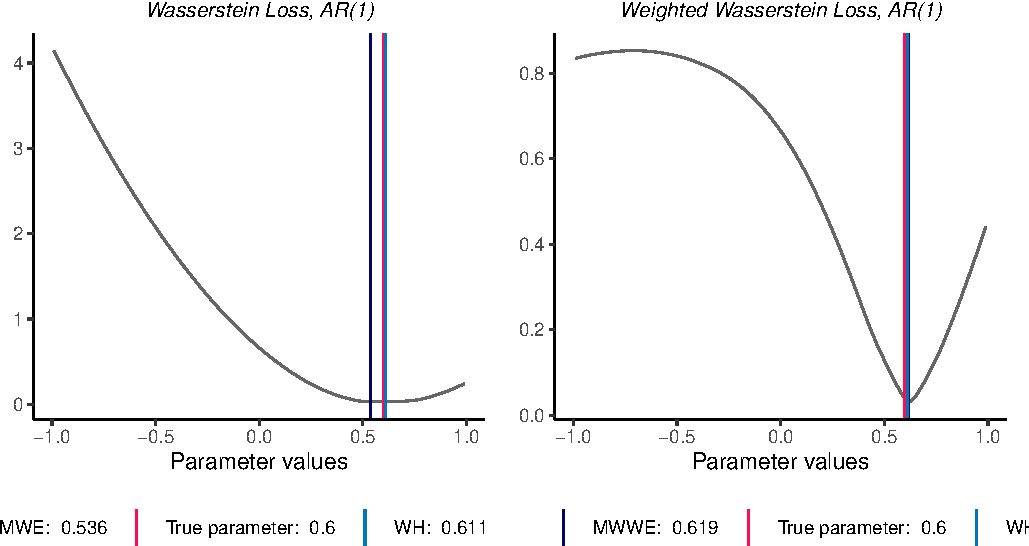
\includegraphics[width=0.7\linewidth]{Master_thesis_V1_files/figure-latex/wass_ar1-1} 

}

\caption{Wasserstein loss and weighted Wasserstein loss functions of a Gaussian AR(1) process. The sample size is 3001 and the true parameter is 0.6.}\label{fig:wass_ar1}
\end{figure}

\hypertarget{minimum-sinkhorn-estimator}{%
\subsubsection{Minimum Sinkhorn
Estimator}\label{minimum-sinkhorn-estimator}}

A second idea is to employ the Sinkhorn divergence (see Eq.
\ref{eq:sink}) to estimate our parameter based on
\protect\hyperlink{ref-cuturi2013sinkhorn}{Cuturi}
(\protect\hyperlink{ref-cuturi2013sinkhorn}{2013}). The regularization
term should make the loss function smoother. On Figure
\ref{fig:sinkhorn}, we compare the loss function when we employ the
Wasserstein distance or the Sinkhorn divergence to estimate our
parameter. Indeed, we end up with a smooth and concave function. The
reached minimum is very close to the true value. A good property with
the Sinkhorn divergence is that it remains smooth even for a very small
sample size.

\hfill\break
\hfill\break

\begin{center}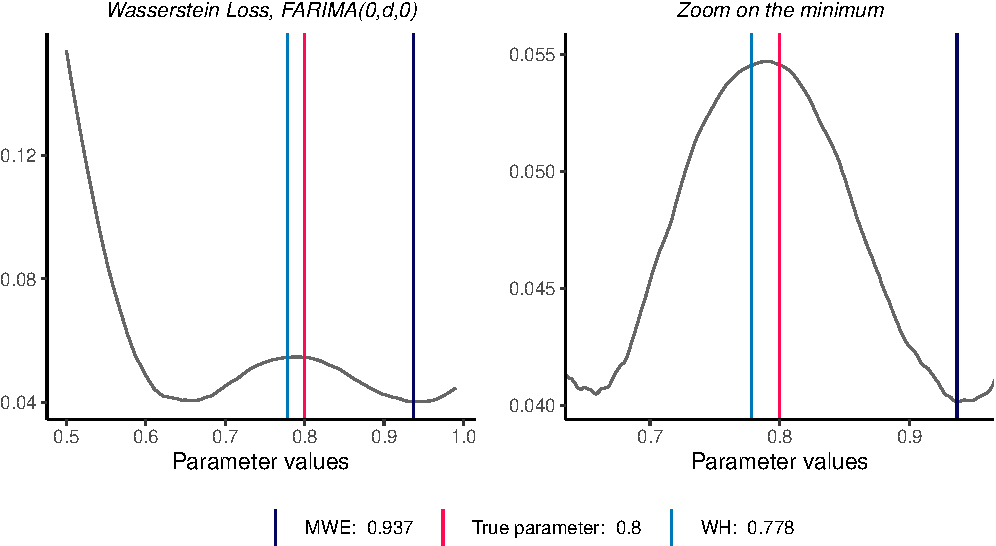
\includegraphics[width=0.65\linewidth]{Master_thesis_V1_files/figure-latex/wasserstein_SH-1} \end{center}

\begin{figure}

{\centering 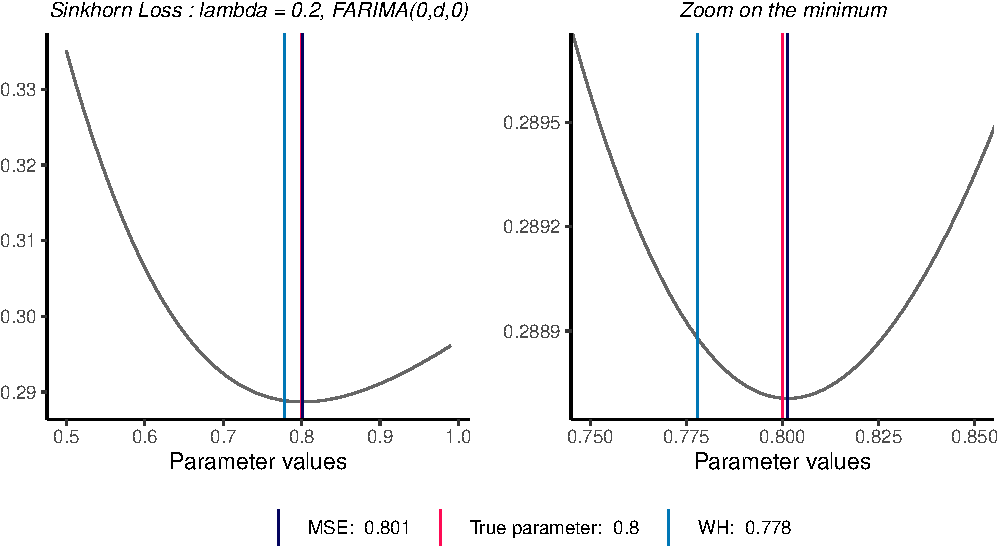
\includegraphics[width=0.65\linewidth]{Master_thesis_V1_files/figure-latex/sinkhorn-1} 

}

\caption{Top: Wasserstein loss function of a FARIMA(0,d,0) process. Bottom: Sinkhorn loss function of the same process. The sample size is 1801.}\label{fig:sinkhorn}
\end{figure}

Following this, we are confronted to an important choice: which values
to select for \(\lambda\)? As a reminder, when \(\lambda\) is very
small, the Sinkhorn divergence approximates the Wasserstein distance. In
order to choose the optimal lambda we suggest to implement classical
machine learning techniques to perform model selection such as cross
validation, leave-one-out, etc. For more information see for example
\protect\hyperlink{ref-friedman2001elements}{Friedman et al.}
(\protect\hyperlink{ref-friedman2001elements}{2001}) Chapter 7.

For instance, we randomly divide a time series into \(2\) groups
\(C_1 \ (80\%), C_2 \ (20\%)\) also called folds. We treat the first
group as train and the second group as validation/test. For a selection
of \(\lambda\), we estimate our MSE parameter on the train set and then
use the corresponding \(\hat \theta_{MSE}\) to predict the time data of
our test set. For simplicity, we demonstrate the procedure with an AR(1)
process, \(Y_t = \phi_1 Y_{t-1} + \epsilon_t\) where
\(\epsilon_t \sim N(0,1)\) and \(\theta^* = \phi_1 = 0.6\). After
estimating the parameter thanks to the train set, we substitute its
value in \(\hat \epsilon_t = Y_t - \hat \theta^*_{MSE} Y_{t-1}\) where
\(t = 2, ..., l\). \(l\) is the length of the testing vector and depends
on which ratios we choose to split our time process \({Y_t}\) in our
case \(80\% - 20\%\). Then, we use the predictions of the error terms to
compute the Mean Squared Errorfor a given \(\lambda\):

\[MSE_{\lambda} \textit{ of the test set} = \frac{1}{l}\sum_{t = 2}^l \hat \epsilon_t = \frac{1}{l} \sum_{t = 2}^l (Y_t - \hat \theta^*_{MSE} Y_{i-t})\]

We repeat this method for several lambda values and plot the results on
Figure \ref{fig:SH_CV}. The minimum testing error is achieved when
\(\lambda = 0.1\) given an estimate
\(\hat \theta^*_{MSE_{\lambda = 0.1}} = 0.572\) which is close to the
true parameter value \(\theta^* = 0.6\).

\begin{figure}

{\centering 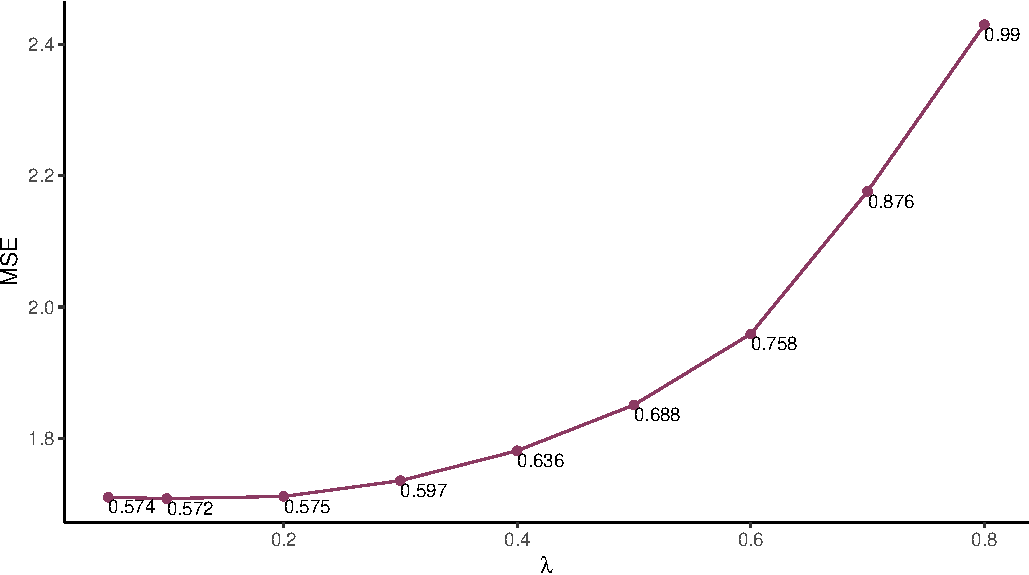
\includegraphics[width=0.75\linewidth]{Master_thesis_V1_files/figure-latex/SH_CV-1} 

}

\caption{Testing MSE vs lambda values for an AR(1) process. The sample size is  4001 and the true parameter value is 0.6. For this process, the minimum MSE is achieved when lambda = 0.1.}\label{fig:SH_CV}
\end{figure}

\hypertarget{results}{%
\section{Results}\label{results}}

\hypertarget{monte-carlo-simulations}{%
\subsection{Monte Carlo Simulations}\label{monte-carlo-simulations}}

Our criterion for evaluating the performance of each of the estimators
is, as it is often the case in machine learning, the Mean Squared Error
(\(MSE\))

\[MSE(\hat \theta^*, \theta^*) = \sum^{mt}(\hat \theta^* - \theta^*)^2 \approx \operatorname{Var}(\hat{\theta^*})+\operatorname{Bias}^{2}(\hat{\theta^*})\]

where \(mt\) is the number of Monte Carlo simulations, i.e.~the number
of simulated processes. The MSE represents the bias-variance trade-off
which typically emerges in statistics when it comes to model selection.

\hypertarget{long-memory-process}{%
\subsubsection{Long-memory Process}\label{long-memory-process}}

Firstly, we simulate \(mt = 200\) stationary FARIMA(\(0,d,0\)) processes
of size \(n = 3201\) according to

\[(1-L)^{1.3}Y_t = \epsilon_t.\]

For each process, we compute the Whittle's estimator
\(\hat \theta^*_{WH}\), the minimum Wasserstein estimator
\(\hat \theta^*_{MWE}\), the mean of the minimum Wasserstein estimators
\(\hat \theta^*_{MMWE}\), the minimum semidiscrete Wasserstein estimator
\(\hat \theta^*_{MSWE}\), the minimum weighted Wasserstein estimator
\(\hat \theta^*_{MWWE}\) and the minimum Sinkhorn estimator
\(\hat \theta^*_{MSE}\). Figure \ref{fig:box_farima_t200} reports the
results. We can observe that, due to the random form of the Wasserstein
loss function, we have an estimator with a very large variance. As
expected, by using either the mean of the minimum Wasserstein estimators
or the true cumulative distribution function, we can reduce the
variance. The most important results concern the MWWE and MSE. Indeed,
both new estimators have small variance and no bias (at least, similar
to the Whittle's estimator).The MWWE estimator is very close to the
Whittle estimator in terms of MSE (see Table
\ref{tab:farima_mse_gaussian}). Both new estimators have small variance
and no bias.

\begin{figure}

{\centering 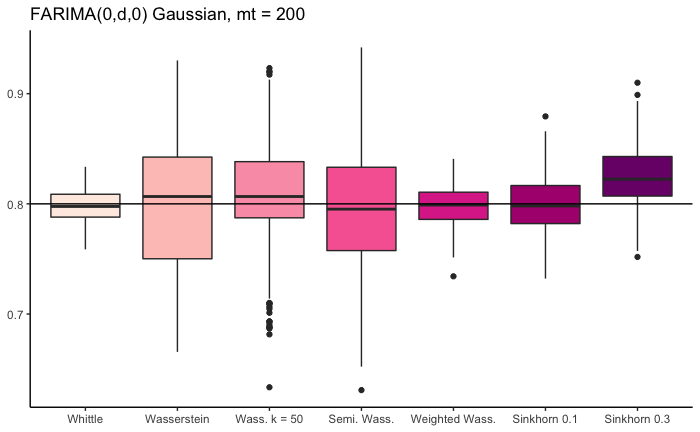
\includegraphics[width=0.75\linewidth]{/Users/manonfelix/OneDrive/Master thesis/Redaction/images/box_farima_t200} 

}

\caption{Boxplots of all the estimators presented during this thesis. The sample size of the 200 simulated FARIMA(0,d,0) is 3201.}\label{fig:box_farima_t200}
\end{figure}

An important point to note is that the estimation depends a lot on the
vector \(Z_j\). On Figure \ref{fig:box_farima_t200} each process is
compared to a new vector \(Z_j\). So we have a total of 200 time series
and 200 vectors \(Z_j\). For the sake of the example, we now simulate
200 FARIMA(\(0,d,0\)) processes again and compare them all to the same
unique vector \(Z_j\). This leads to the graph in Figure
\ref{fig:box_farima_t1} and the corresponding MSE in Table
\ref{tab:farima_mse_gaussian}. With this vector, for example, the MWWE
and the MSE (\(\lambda = 0.1\)) overperform the Whittle's estimator in
terms of MSE.

\begin{figure}

{\centering 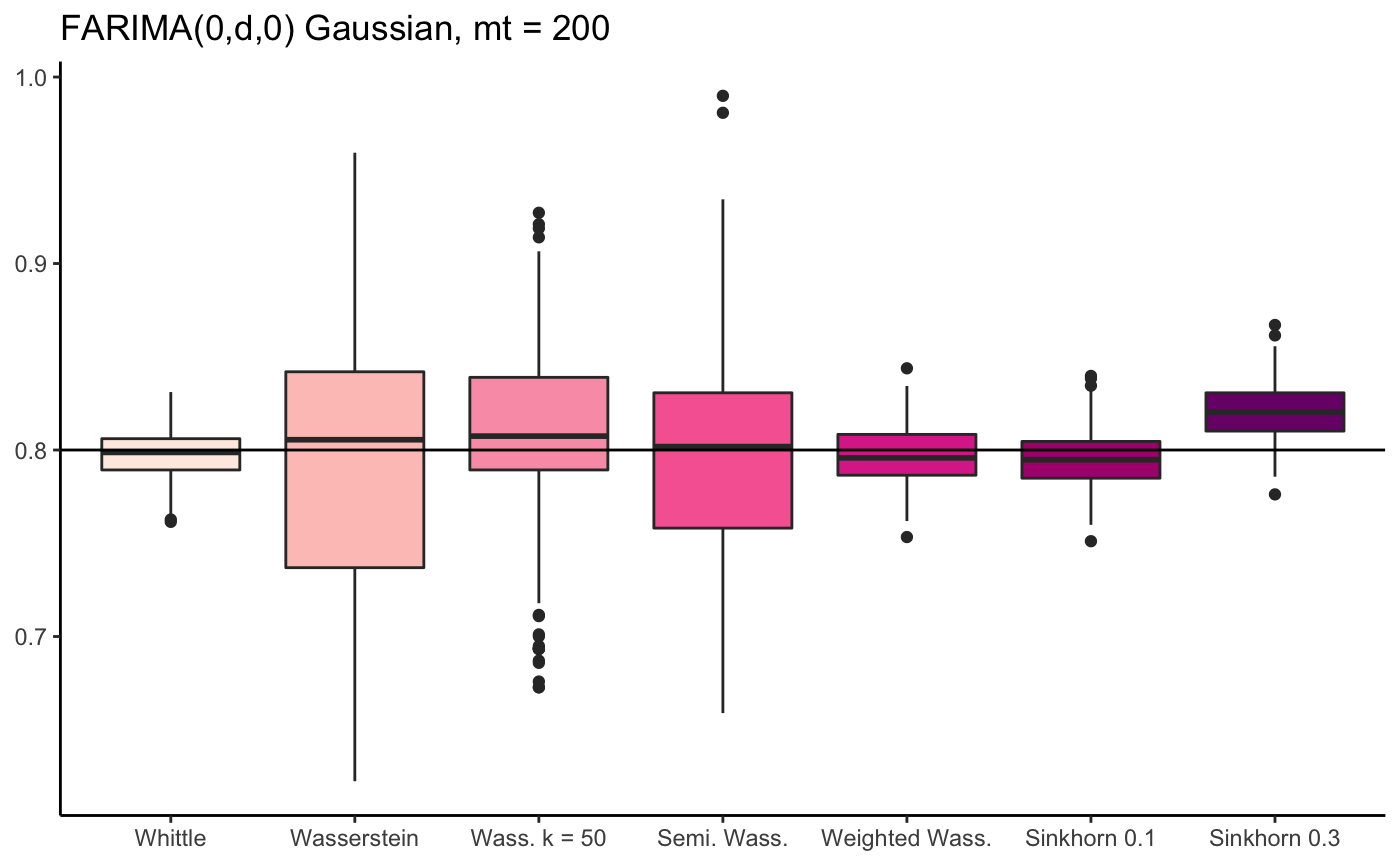
\includegraphics[width=0.75\linewidth]{/Users/manonfelix/OneDrive/Master thesis/Redaction/images/boxplot_farima_t1} 

}

\caption{Boxplots of all the estimators presented during this thesis. The sample size of the 200 simulated FARIMA(0,d,0) is 3201. All the estimators are computed using a unique random vector.}\label{fig:box_farima_t1}
\end{figure}

\begin{table}[h]
\centering
\begin{tabular}{|c|c|c|}
\hline
\textbf{MSE}          & \textit{\textbf{d}}                  & \textit{\textbf{d}}                    \\ \hline
\textbf{Distribution} & \textbf{Gaussian with 200 vectors Z} & \textbf{Gaussian with unique vector Z} \\ \hline
Whittle               & 7.921                                & 7.861                                  \\ \hline
MWE                   & 8.692                                & 8.322                                  \\ \hline
MMWE, k = 50          & 9.191                                & 9.281                                  \\ \hline
MSWE                  & 8.326                                & 8.313                                  \\ \hline
MWWE                  & 7.933                                & 7.822                                  \\ \hline
MSE 0.1               & 8.095                                & 7.699                                  \\ \hline
MSE 0.3               & 10.729                               & 9.8352                                 \\ \hline
\end{tabular}
\caption{Mean Squared Errors of Figure 10. and 11.}
\label{tab:farima_mse_gaussian}
\end{table}

\hypertarget{heavy-tailed-distribution}{%
\paragraph{Heavy-tailed Distribution}\label{heavy-tailed-distribution}}

\hfill\break

Mikosch et al.~(1995) showed that the fatter the tails of the innovation
distributions, the faster the Whittle's estimator converges to the true
parameter value. Regarding the Wasserstein loss function, it becomes
smooth and concave when the error distribution is heavy-tailed (see
Figure \ref{fig:student_t}), even for small sample sizes. Therefore, the
Whittle's estimator and the MWE are often very close, unbiased and with
small variances.

\begin{figure}

{\centering 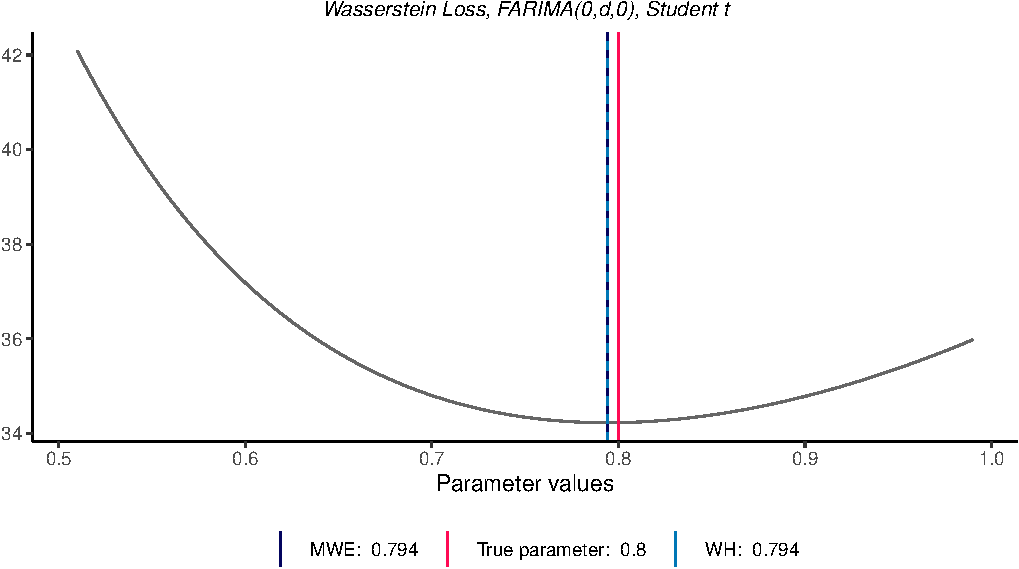
\includegraphics[width=0.6\linewidth]{Master_thesis_V1_files/figure-latex/student_t-1} 

}

\caption{Wasserstein loss function of a FARIMA(0,d,0) process distributed according to a Student t distribution with degree of freedom equal to 2. The sample size is equal to 3001.}\label{fig:student_t}
\end{figure}

We simulate again \(mt = 200\) FARIMA(0,d,0) processes with, this time,
a Student t underlying distribution with degree of freedom equal to 2.
On Figure \ref{fig:box_farima_student}, we note that all estimators
(apart from those based on the Sinkhorn distance) have indeed a very
small variance and are mostly unbiased. The weighted wasserstein
distance is irrelevant and all the minimum Sinhorn estimators (see Table
\ref{tab:FARIMA_heavy_MSE}) are similar.

\begin{figure}

{\centering 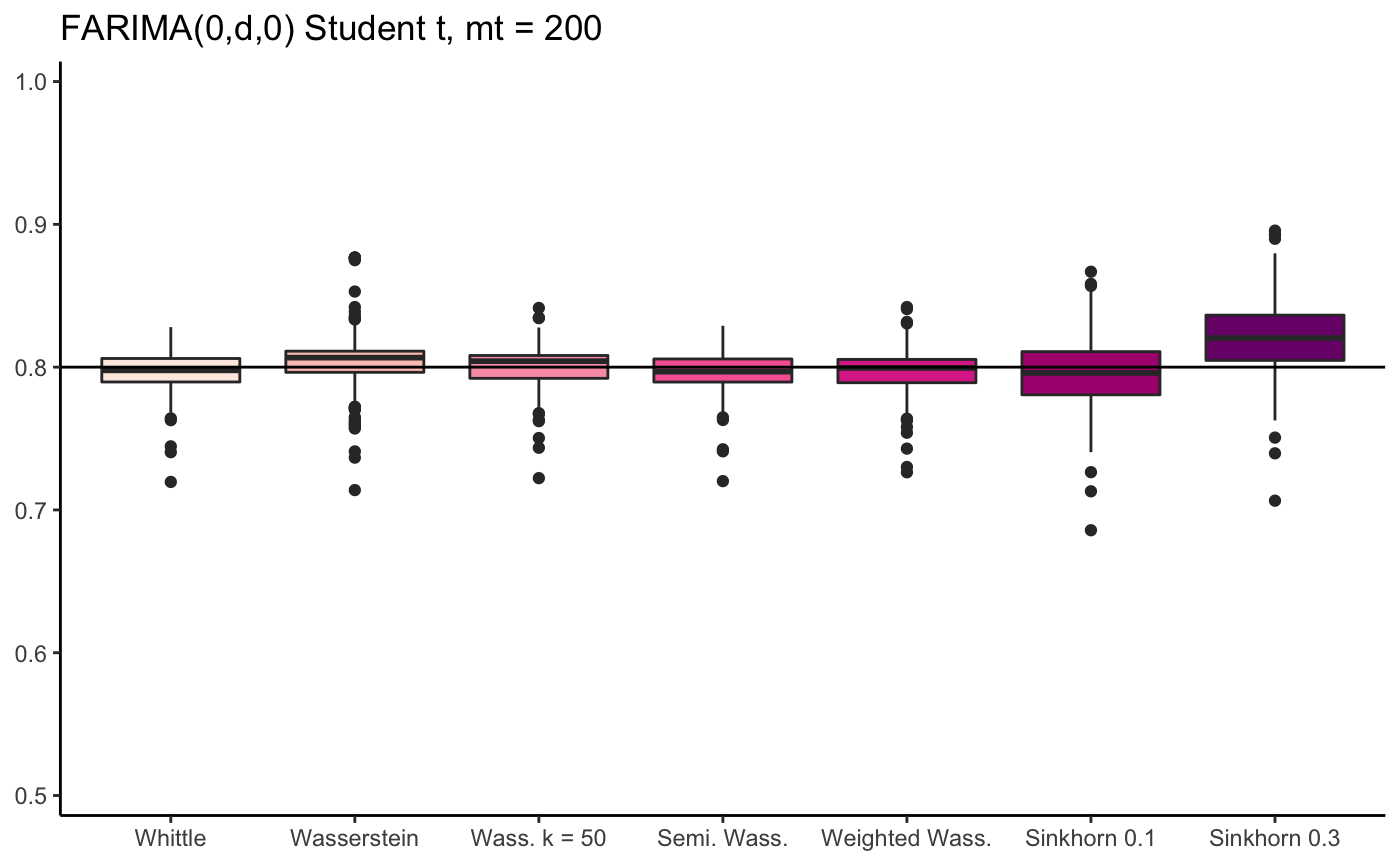
\includegraphics[width=0.75\linewidth]{/Users/manonfelix/OneDrive/Master thesis/Redaction/images/boxplot_farima_student} 

}

\caption{Boxplots of all the estimators presented during this thesis. The sample size of the 200 simulated FARIMA(0,d,0) is 3201 and the underlying distribution is a Student t with degree of freedom equal to 2.}\label{fig:box_farima_student}
\end{figure}

Let us now focus on the case where the distribution of the innovation
terms is skewed. The skew t distribution was recently developed by
\protect\hyperlink{ref-azzalini2003distributions}{Azzalini and
Capitanio} (\protect\hyperlink{ref-azzalini2003distributions}{2003}). It
is related to a standard skew normal random variable \(Z\) and a random
variable \(W\) following a chi-squared distribution with \(\nu\) degree
of freedom by the equation:

\[Y=\frac{Z}{\sqrt{\frac{W}{\nu}}}.\]

Then the linear transformation \(X=\mu+\sigma Y\) has a skew-t
distribution with parameters \(\mu, \sigma, \alpha\), and \(\nu\) and
the corresponding notation \(S T(\mu = 0, \sigma = 1, \gamma, \nu)\) to
denote the skew t random variable \(X\). For example, we consider the
underlying distribution of the process as a skew t distribution with
degree of freedom equal to 2 and skewness parameter \(\gamma\) equal to
4 (see Figure \ref{fig:skewt_density}).

\begin{figure}

{\centering 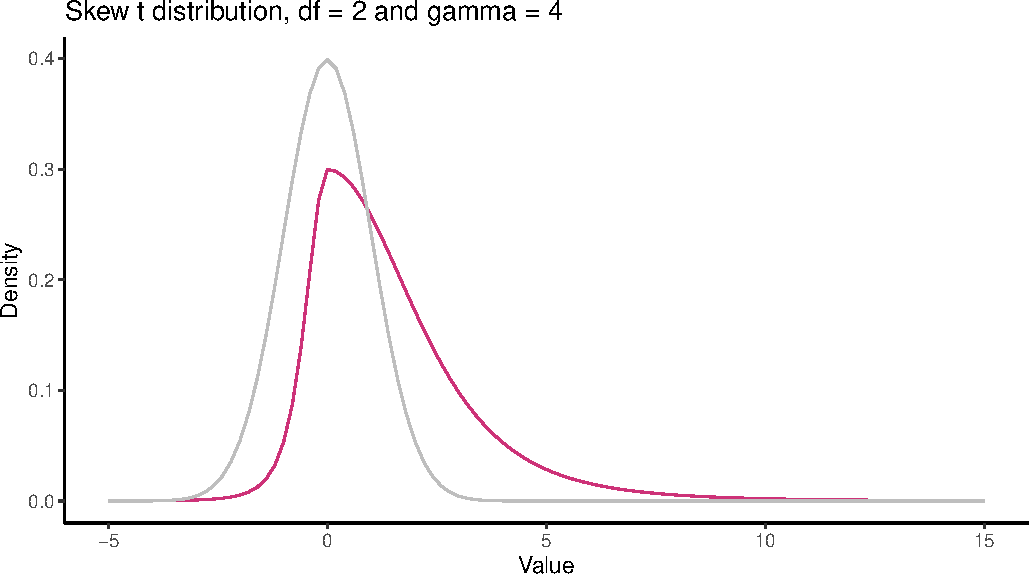
\includegraphics[width=0.5\linewidth]{Master_thesis_V1_files/figure-latex/skewt_density-1} 

}

\caption{Skew t distribution with degree of freedom = 2 and gamma = 4.}\label{fig:skewt_density}
\end{figure}

The Wasserstein loss function is still smooth and concave (see Figure
\ref{fig:skew_t}).

\begin{figure}

{\centering 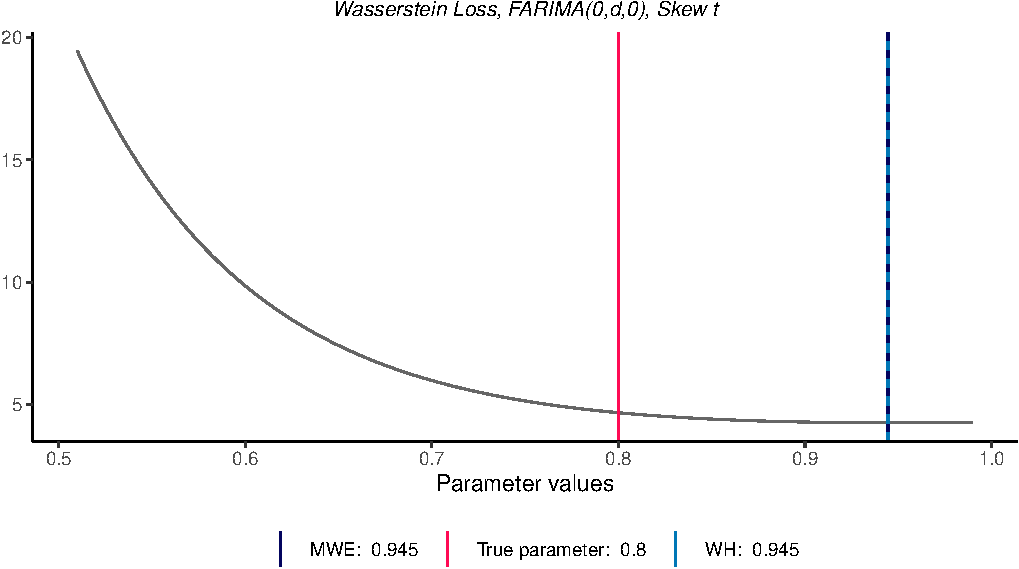
\includegraphics[width=0.6\linewidth]{Master_thesis_V1_files/figure-latex/skew_t-1} 

}

\caption{Wasserstein loss function of a FARIMA(0,d,0) process distributed according to a skew t distribution with degree of freedom = 4 and gamma = 2. The sample size is equal to 3001.}\label{fig:skew_t}
\end{figure}

As we can see on Figure \ref{fig:box_farima_skewt}, all estimators are
biased and overestimate the value of the parameter. Regarding the MSE
values listed in Table \ref{tab:FARIMA_heavy_MSE}, all our new
estimators surpass the Whittle's estimator except for the MWWE which is
irrelevant. The gain is principally in terms of bias.

\hfill\break

\begin{figure}[h]

{\centering 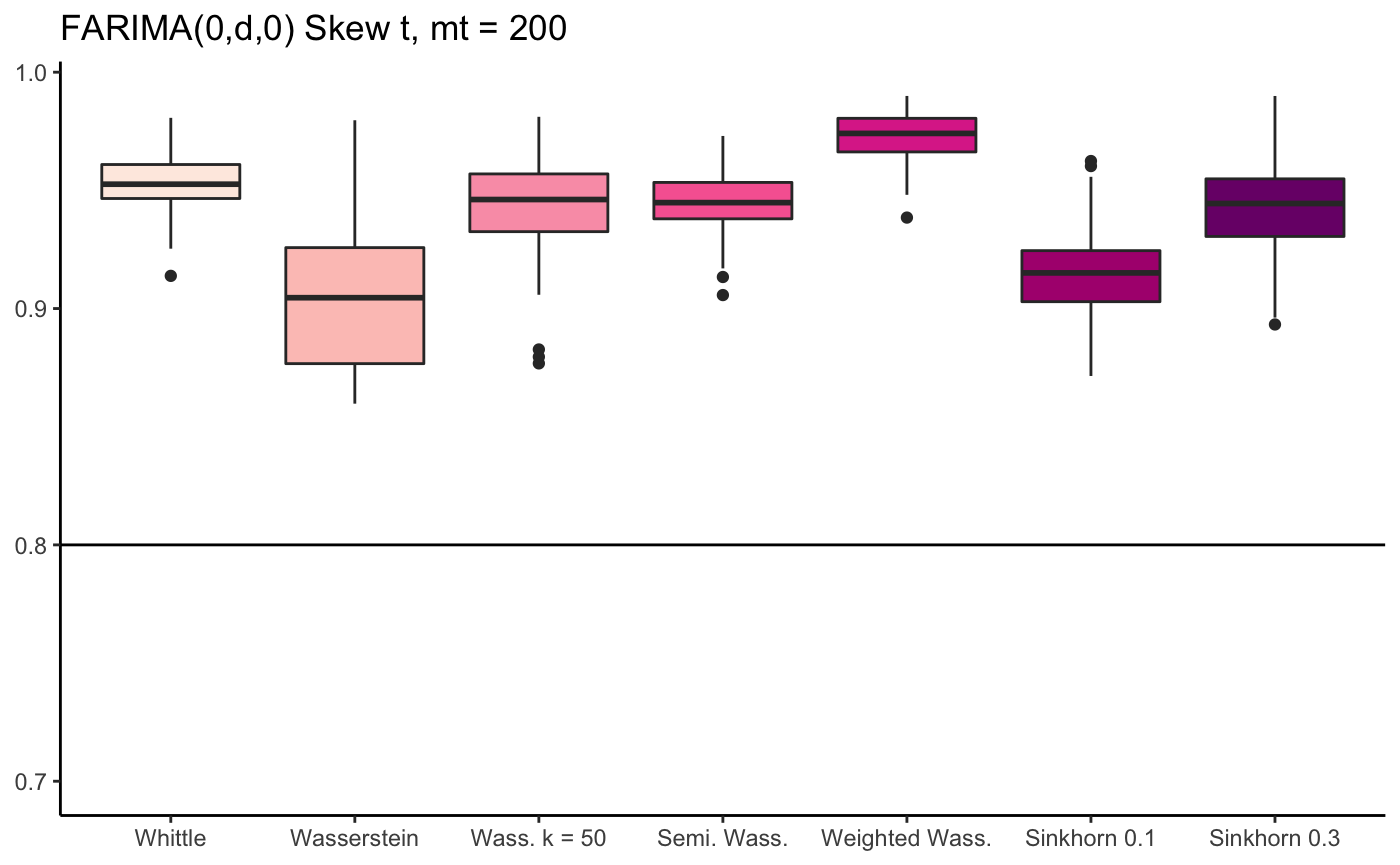
\includegraphics[width=0.75\linewidth]{/Users/manonfelix/OneDrive/Master thesis/Redaction/images/boxplot_farima_skewt} 

}

\caption{Boxplots of all the estimators presented during this thesis. The sample size of the 200 simulated FARIMA(0,d,0) is 3201 and the underlying distribution is a skew t with df = 4 and gamma = 2.}\label{fig:box_farima_skewt}
\end{figure}

\begin{table}[h]
\centering
\begin{tabular}{|c|c|c|}
\hline
\textbf{MSE}          & \textit{\textbf{d}} & \textit{\textbf{d}} \\ \hline
\textbf{Distribution} & \textbf{Student t}  & \textbf{Skew t}     \\ \hline
Whittle               & 7.768               & 24.906              \\ \hline
MWE                   & 7.850               & 18.708              \\ \hline
MMWE, k = 50          & 8.058               & 23.761              \\ \hline
MSWE                  & 7.754               & 23.826              \\ \hline
MWWE                  & 8.485               & 27.889              \\ \hline
MSE 0.1               & 7.815               & 19.848              \\ \hline
MSE 0.3               & 9.944               & 23.590              \\ \hline
\end{tabular}
\caption{Mean Squared Error of Figure 13 and 16.}
\label{tab:FARIMA_heavy_MSE}
\end{table}

\hypertarget{additive-outliers}{%
\paragraph{Additive Outliers}\label{additive-outliers}}

\hfill\break

In the presence of contamination in the time series (e.g.~additive
outliers). For in example, in the case of Gaussian FARIMA(0, d, 0) some
of our estimators (in particular, the ones based on weighted Wasserstein
distance and/or on the Sinkhorn divergence) seem to overperform
Whittle's estimator in terms of MSE. To demonstrate this propriety we
simulate \(mt = 200\) FARIMA(\(0,d,0\)) contaminated by occasional
isolated outliers. The processes \(\{Y_t\}\) are distributed according
to

\[Y_{t}=\left(1-W_{t}\right) X_{t}+W_{t}\left(c \cdot V_{t}\right)\]
where \(W_t \sim Bern(p)\), \(V_t \sim t_2\) and c = 10. In Table
\ref{tab:outliers}, we report the ratio between the MSE of the Whittle's
estimator and the minimum weighted Wasserstein estimator for different
values of \(p\). The results suggest that when the time series is
contaminated, the MWWE overperform the Whittle's estimator in terms of
MSE.

\begin{table}[h]
\centering
\begin{tabular}{|c|c|c|c|c|}
\hline
p  &  0  & 0.001   & 0.01    & 0.05 \\
\hline
ratio  & 0.682 & 1.208 & 1.105 & 1.018939 \\
\hline
\end{tabular}
\caption{MSE of the Whittle's estimator divided by the MSE of the MWWE. The number of simulated time series is equal to 200 with sample size equal to 3001.}
\label{tab:outliers}
\end{table}

\hypertarget{short-memory-process}{%
\subsubsection{Short-memory Process}\label{short-memory-process}}

We also aim to demonstrate the performance of our estimators for
short-memory processes. To do this, we simulate \(mt = 200\)
auto-regressive processes of order 2 according to:

\[Y_t = 0.75 Y_{t-1} - 0.25Y_{t-2} + \epsilon_t.\]

The processes are stationary since the three stationary conditions are
met:

\begin{enumerate}
\def\labelenumi{\arabic{enumi}.}
\tightlist
\item
  \(\phi_{2}<1+\phi_{1}\)
\item
  \(\phi_{2}<1-\phi_{1}\)
\item
  \(\phi_{2}>-1\)
\end{enumerate}

where \(\phi_1 = 0.75\) and \(\phi_2 = -0.25\).

We cannot include the Sinkhorn divergence in our comparison because the
function used on R requires too much time to calculate this divergence
and fails to converge. The results when
\(\theta^* \subset \mathbb{R}^2\) are on Figure \ref{fig:box_ar2} with
corresponding MSE in Table \ref{tab:AR2_mse_table}. Again, we consider
several distributions for \(\epsilon_t\):
\(\epsilon_t \sim N(0,1), \epsilon_t \sim t_2\) and
\(\epsilon_t \sim S T(\mu = 0, \sigma = 1, \gamma = 2, \nu = 4)\)

\begin{center}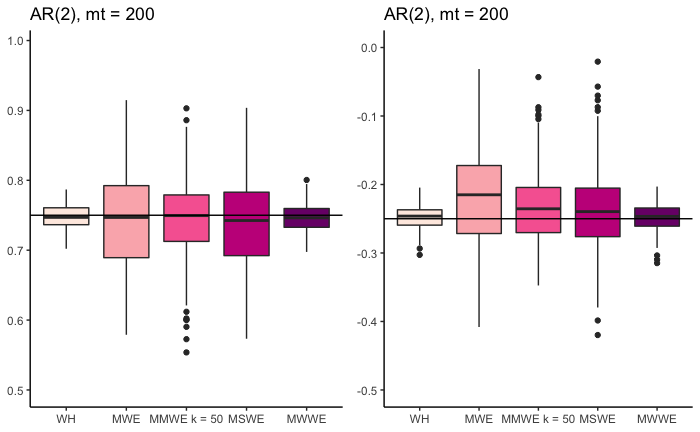
\includegraphics[width=0.6\linewidth]{/Users/manonfelix/OneDrive/Master thesis/Redaction/images/AR2_gauss} \end{center}

\begin{center}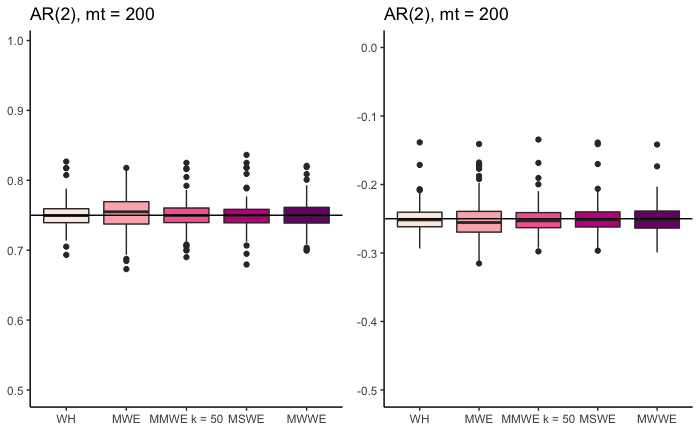
\includegraphics[width=0.6\linewidth]{/Users/manonfelix/OneDrive/Master thesis/Redaction/images/AR2_student} \end{center}

\begin{figure}

{\centering 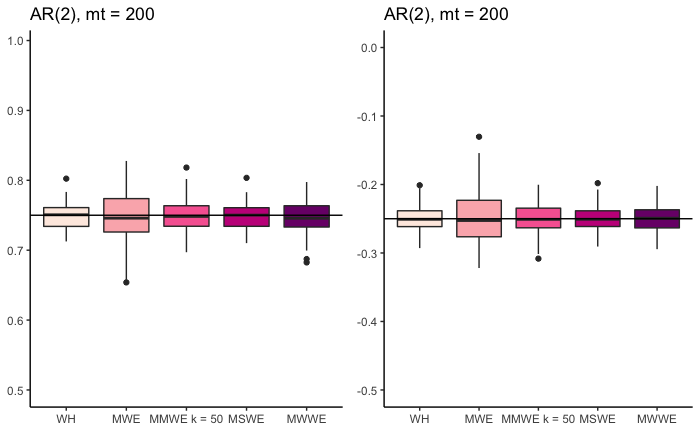
\includegraphics[width=0.6\linewidth]{/Users/manonfelix/OneDrive/Master thesis/Redaction/images/AR2_skewt} 

}

\caption{Boxplots of the Whittle's estimator, MWE, MSWE, MMWE, MWWE for 200 AR(2) processes. The innovation terms densities are (in the order of apparition): Gaussian, Student t, Skew t. The left column is the first parameter (0.75) of the process, the right one is for the second parameter (-0.25).}\label{fig:box_ar2}
\end{figure}

When the process is Gaussian, the MSE of the minimum weighted
Wasserstein estimator is similar to Whittle's estimator. The other
estimators have large variance. As observed for processes with
long-memory, when the tails of the error distributions are wider than
those of the normal distribution, the MWE converges to Whittle's
estimator. In this case, all estimators are relatively similar in terms
of MSE (bias - variance). On the other hand, contrary to long-memory
processes, when we work with short-memory processes we observe that the
fact that the underlying distribution are skewed or not is not relevant
during the estimation procedure. Indeed, the results for the Student t
and the skew t distribution are very close.

\begin{table}[h]
\centering
\begin{tabular}{|l|c|c|c|c|c|c|}
\hline
\textbf{MSE}          & $\phi_1$           & $\phi_2$          & $\phi_1$           & $\phi_2$           & $\phi_1$          & $\phi_2$         \\ \hline
\textbf{Distribution} & \multicolumn{2}{l|}{\textbf{Gaussian}} & \multicolumn{2}{l|}{\textbf{Student t}} & \multicolumn{2}{l|}{\textbf{Skew t}} \\ \hline
Whittle               & 0.052              & 0.059             & 0.061              & 0.067              & 0.061             & 0.060            \\ \hline
MWE                   & 1.024              & 1.345             & 0.134              & 0.139              & 0.255             & 0.290            \\ \hline
MMWE, k = 50          & 0.690              & 0.652             & 0.073              & 0.087              & 0.087             & 0.087            \\ \hline
MSWE                  & 0.885              & 0.897             & 0.073              & 0.083              & 0.062             & 0.061            \\ \hline
MWWE                  & 0.070              & 0.083             & 0.078              & 0.084              & 0.091             & 0.079            \\ \hline
\end{tabular}
\caption{Mean Squared Error of Figure 17.}
\label{tab:AR2_mse_table}
\end{table}

\hypertarget{conclusion}{%
\section{Conclusion}\label{conclusion}}

To conclude, we introduce, in this thesis, five new estimators that are
based on minimum distance estimation. Our results suggest that we can
outperform the state-of-the art estimation procedure when we are dealing
with long-memory processes that have skewed underlying distributions.
Moreover, it seems that our minimum weighted Wasserstein estimator can
also be more efficient when the process is contaminated by occasional
outliers. In the case of short memory processes, we have similar results
to Whittle's estimator in terms of MSE. Through this thesis, we open the
possibility for further research. Indeed, the weights are certainly not
optimal and therefore would be subject to further investigation. As well
as the choice of the regularization parameter when using the Sinkhorn
divergence. The shape of the Wasserstein loss function and why the
estimation procedure behaves better for certain vector \(Z_j\) also
remains an opened question. We can also extend our research to other
distances such as the energy distance:

\[D^{2}(F, G)=2 \int_{-\infty}^{\infty}(F(t)-G(t))^{2} \mathrm{~d} t.\]
Another important step is to compute the theory surrounding these
estimators (consistency, robustness, etc.). To sum up, our results are
promising and open the possibility of further researches.

\newpage

\hypertarget{references}{%
\section*{References}\label{references}}
\addcontentsline{toc}{section}{References}

\hypertarget{refs}{}
\begin{CSLReferences}{1}{0}
\leavevmode\hypertarget{ref-arjovsky2017wasserstein}{}%
Arjovsky, Martin, Soumith Chintala, and Léon Bottou. 2017.
{``Wasserstein Generative Adversarial Networks.''} In
\emph{International Conference on Machine Learning}, 214--23. PMLR.

\leavevmode\hypertarget{ref-azzalini2003distributions}{}%
Azzalini, Adelchi, and Antonella Capitanio. 2003. {``Distributions
Generated by Perturbation of Symmetry with Emphasis on a Multivariate
Skew t-Distribution.''} \emph{Journal of the Royal Statistical Society:
Series B (Statistical Methodology)} 65 (2): 367--89.

\leavevmode\hypertarget{ref-bassetti2006minimum}{}%
Bassetti, Federico, Antonella Bodini, and Eugenio Regazzini. 2006. {``On
Minimum Kantorovich Distance Estimators.''} \emph{Statistics \&
Probability Letters} 76 (12): 1298--1302.

\leavevmode\hypertarget{ref-basu2019statistical}{}%
Basu, Ayanendranath, Hiroyuki Shioya, and Chanseok Park. 2019.
\emph{Statistical Inference: The Minimum Distance Approach}. Chapman;
Hall/CRC.

\leavevmode\hypertarget{ref-beran1994statistics}{}%
Beran, Jan. 1994. \emph{Statistics for Long-Memory Processes}. Vol. 61.
CRC press.

\leavevmode\hypertarget{ref-bernton2019parameter}{}%
Bernton, Espen, Pierre E Jacob, Mathieu Gerber, and Christian P Robert.
2019. {``On Parameter Estimation with the Wasserstein Distance.''}
\emph{Information and Inference: A Journal of the IMA} 8 (4): 657--76.

\leavevmode\hypertarget{ref-brillinger2001time}{}%
Brillinger, David R. 2001. \emph{Time Series: Data Analysis and Theory}.
SIAM.

\leavevmode\hypertarget{ref-cuturi2013sinkhorn}{}%
Cuturi, Marco. 2013. {``Sinkhorn Distances: Lightspeed Computation of
Optimal Transport.''} \emph{Advances in Neural Information Processing
Systems} 26: 2292--2300.

\leavevmode\hypertarget{ref-friedman2001elements}{}%
Friedman, Jerome, Trevor Hastie, Robert Tibshirani, and others. 2001.
\emph{The Elements of Statistical Learning}. Vol. 1. 10. Springer series
in statistics New York.

\leavevmode\hypertarget{ref-kantorovich1942translocation}{}%
Kantorovich, Leonid V. 1942. {``On the Translocation of Masses.''} In
\emph{Dokl. Akad. Nauk. USSR (NS)}, 37:199--201.

\leavevmode\hypertarget{ref-monge1781memoire}{}%
Monge, Gaspard. 1781. {``M{é}moire Sur La Th{é}orie Des d{é}blais Et Des
Remblais.''} \emph{Histoire de l'Acad{é}mie Royale Des Sciences de
Paris}.

\leavevmode\hypertarget{ref-ni2020conditional}{}%
Ni, Hao, Lukasz Szpruch, Magnus Wiese, Shujian Liao, and Baoren Xiao.
2020. {``Conditional Sig-Wasserstein GANs for Time Series Generation.''}
\emph{arXiv Preprint arXiv:2006.05421}.

\leavevmode\hypertarget{ref-panaretos2019statistical}{}%
Panaretos, Victor M, and Yoav Zemel. 2019. {``Statistical Aspects of
Wasserstein Distances.''} \emph{Annual Review of Statistics and Its
Application} 6: 405--31.

\leavevmode\hypertarget{ref-priestley1981spectral}{}%
Priestley, Maurice Bertram. 1981. \emph{Spectral Analysis and Time
Series: Probability and Mathematical Statistics}. 04; QA280, P7.

\leavevmode\hypertarget{ref-tsay2005analysis}{}%
Tsay, Ruey S. 2005. \emph{Analysis of Financial Time Series}. Vol. 543.
John wiley \& sons.

\leavevmode\hypertarget{ref-whittle1953estimation}{}%
Whittle, Peter. 1953. {``Estimation and Information in Stationary Time
Series.''} \emph{Arkiv f{ö}r Matematik} 2 (5): 423--34.

\end{CSLReferences}

\end{document}
